\section{实验}
\subsection{实验设置}

\begin{table*}[t]
\begin{center}
\begin{tabular}{ >{\raggedright\arraybackslash}p{3.9cm} c c c c c c c c }
    \toprule

    \textbf{[调整过的] 模型} & \textbf{方法} & \bm{$K$} & \textbf{有帮助} & \textbf{清晰} & \textbf{事实性} & \textbf{深度} & \textbf{参与度} & \textbf{平均} \\
    \midrule

    [\xmark] Mistral 7b  & 基础 & 0 & 2.20 & 2.51 & 2.29 & 1.69 & 1.80 & 2.10 \\

   [\xmark] Mistral 7b  & URIAL & 3 & 3.62 & 4.32 & 3.75 & 2.70 & 3.41 &  3.56\\

    [\xmark] Mistral 7b  & \ours & 2 & \textbf{4.23} & \textbf{4.56} & \textbf{3.97} & \textbf{3.68} & \textbf{3.84} &  \textbf{4.06}\\

    \hline

   [\cmark] Mistral 7b (Instruct) & 基础 & 0 & 3.98 & 4.44 & 3.64 & 2.97 & 3.26 &  3.66\\

   [\cmark] Mistral 7b (Instruct) & URIAL & 3 & 3.94 & 4.51 & 3.69 & 2.99 & 3.75 &  3.78\\

    [\cmark] Mistral 7b (Instruct) & \ours & 2 & \textbf{4.22} & \textbf{4.60} & \textbf{3.80} & \textbf{3.68} & \textbf{3.99} &  \textbf{4.06}\\

   \hline

    [\xmark] Llama 2 70b$^q$  & 基础 & 0 & 2.07 & 2.55 & 2.35 & 1.50 & 1.63 &  2.02 \\

    [\xmark] Llama 2 70b$^q$ & URIAL & 3 & 4.25 & 4.67 & 4.03 & 3.08 & 3.80 &  3.97 \\

    [\xmark] Llama 2 70b$^q$  & \ours & 2 & \textbf{4.42} & \textbf{4.72} & \textbf{4.23} & \textbf{3.81} & \textbf{3.98} &  \textbf{4.23}\\

    \hline

    [\cmark] Llama 2 70b$^q$ (chat) & 基础 & 0 & 4.36 & 4.71 & 3.95 & 3.56 & 3.76 &  4.07\\

    [\cmark] Llama 2 70b$^q$ (chat) & URIAL & 3 & 4.32 & 4.72 & 4.08 & 3.50 & 4.25 &  4.17\\

    [\cmark] Llama 2 70b$^q$ (chat) & \ours & 2 & \textbf{4.46} & \textbf{4.75} & \textbf{4.10} & \textbf{4.11} & \textbf{4.37} &  \textbf{4.36}\\

\hline

    [\xmark] Llama 3 8b  & 基础 & 0 & 1.82 & 2.27 & 2.20 & 1.38 & 1.48 &  1.83\\

    [\xmark] Llama 3 8b  & URIAL & 3 & 3.94 & \textbf{4.51} & 3.69 & 2.99 & \textbf{3.75} & 3.78 \\

    [\xmark] Llama 3 8b  & \ours & 2 & \textbf{4.02} & 4.40 & \textbf{3.84} & \textbf{3.50} & 3.65 &  \textbf{3.88} \\

   \hline

    [\cmark] Llama 3 8b (Instruct) & 基础 & 0 & 4.43 & 4.72 & 3.98 & 3.45 & 3.76 &  4.07\\

    [\cmark] Llama 3 8b (Instruct) & URIAL & 3 & 4.48 & 4.81 & \textbf{4.19} & 3.55 & 4.27 &  4.26\\

    [\cmark] Llama 3 8b (Instruct) & \ours & 2 & \textbf{4.54} & \textbf{4.81} & 4.16 & \textbf{4.08} & \textbf{4.40} & \textbf{4.40} \\

    \hline

    [\cmark] \texttt{gpt-3.5-turbo} & 基础 & 0 & 4.56 & 4.89 & 4.41 & 3.30 & 3.55 & 4.14 \\

    [\cmark] \texttt{gpt-3.5-turbo} & URIAL & 3 & 4.30 & 4.77 & 4.41 & 3.44 & 4.11 &  4.21\\

    [\cmark] \texttt{gpt-3.5-turbo} & \ours & 2 & \textbf{4.67} & \textbf{4.92} & \textbf{4.53} & \textbf{4.07} & \textbf{4.58} &  \textbf{4.55}\\

   \hline
    [\cmark] \texttt{gpt-4-0613} & 基础 & 0 & \textbf{4.71} & \textbf{4.93} & \textbf{4.52} & 3.49 & 3.53 &  \textbf{4.24} \\

    \bottomrule

\end{tabular}

\caption{在 \texttt{just-eval-instruct} 基准上的表现。``调整过的'' 表示该模型已进行 SFT/RLHF 调整。模型在多个方面进行评估:``有帮助''(帮助程度)、``清晰''(清晰度)、``事实性''(事实性)、``深度''(深度)和``参与度''(参与度)。基础方法表示基本的对齐提示。我们的方法在多个方面和整体上持续优于基础方法。}
\label{tab:main_table}
\vspace{-17pt}
\end{center}
\end{table*}


\noindent \textbf{评估数据集}。
我们使用标准的对齐基准 \texttt{just-eval-instruct}~\cite{Lin2024ReAlign},该基准结合了五个流行的对齐数据集,提供了全面且细致的 LLM 对齐评估。该基准包含 1,000 个示例:前 800 个用于评估模型的有帮助性,其余 200 个用于评估它们的无害性。前 800 个示例根据五个细化的方面进行评估:\textit{有帮助性}、\textit{清晰度}、\textit{事实性}、\textit{深度} 和 \textit{参与度},而剩余的 200 个则使用 \textit{安全性} 方面进行评估。我们使用 GPT-4 Turbo (\texttt{gpt-4-1106-preview}),这是我们实验中可用的最新 GPT-4 模型之一,来使用原始 URIAL 论文中指定的提示~\cite{Lin2024ReAlign}评估这两类示例。评分范围从 1 到 5,表示 ``强烈不同意''、``不同意''、``中立''、``同意'' 和 ``强烈同意''。请注意,我们使用的是比 URIAL 更近期的 GPT-4 版本,从而提高了我们评估管道的严格性和准确性。因此,我们在更新的评估设置下重新进行了 URIAL 的基准测试,以确保所有结果的一致性。

\noindent \textbf{种子样本}。
在使用 \ours 优化系统提示时,我们从种子数据集 $\mathcal{X}$ 中采样,以衡量系统提示在每个时间步骤的对齐性能。该种子数据集由 180 个示例组成,使用 \texttt{AlpacaEval} \cite{alpaca_eval}、\texttt{LIMA} \cite{zhou2024lima} 和 \texttt{HH-RLHF-redteam} \cite{Ganguli2022RedTL} 的数据构建。关于该数据集构建的更多细节,请参见附录 \ref{sec:impl_details}。

\noindent \textbf{模型}。
我们在实验中基准测试了 6 个开源 LLM 模型:Mistral 7b (v0.1)、Mistral 7b (Instruct)~\cite{Jiang2023Mistral7}、Llama 2 70$b^q$、Llama 2 70$b^q$ (chat)(4-bit AWQ~\cite{lin2023awq} 量化模型)~\cite{Touvron2023Llama2O}、Llama 3 8b、Llama 3 8b (Instruct)~\cite{llama3modelcard},以及 2 个闭源模型:OpenAI 的 GPT-3.5 Turbo (\texttt{gpt-3.5-turbo}) 和 GPT-4 (\texttt{gpt-4-0613})。没有 ``chat'' 或 ``instruct'' 标签的模型为基础模型,即未通过 SFT/RLHF 调整。为了评估,我们使用贪婪解码(温度 = 0)以确保可重复性。

\noindent \textbf{基准方法}。
我们首先将 \ours 应用到基础模型中,使得未使用 \ours 的 SFT/RLHF 调整版本成为自然的基准。例如,我们比较 Mistral 7B + \ours 和 Mistral 7b (Instruct)。此外,我们还有两个基准: (1) 基础方法,在不使用 ICL 示例的情况下应用基本提示。 (2) URIAL~\cite{Lin2024ReAlign},我们使用作者提出的提示和 ICL 示例。我们还提供了我们方法的广泛消融基准,例如将搜索算法从 Beam search 更改为 Greedy Search 或 Monte Carlo search,以及使用 ``静态奖励'' 来理解动态奖励的影响。有关这些的详细信息,请参见附录~\ref{sec:impl_details}。

\noindent \textbf{实现细节}。
我们使用 GPT-4-turbo (\texttt{gpt-4-0125-preview}) 作为优化器 $\mathcal{O}$ 和评估器 $\mathcal{E}$,除非另有说明。初始的上下文学习示例集 $\mathcal{I}_{base}$ 包含 16 个示例:3 个来自 URIAL \cite{Lin2024ReAlign} 和 13 个由 \texttt{gpt-4-0125-preview} 生成的示例。关于 $\mathcal{I}_{base}$ 设计选择的更多细节,请参见附录 \ref{sec:impl_details}。我们使用句子变换器 \cite{reimers-2019-sentence-bert} 从 $\mathcal{I}^*$ 中检索 K 个上下文学习示例。我们使用 $D$ 作为 beam 深度,$W$ 作为 beam 宽度,以及 $M$ 作为每个状态的动作样本数量(用于增长下一个迭代的树)。关于精确超参数的更多信息,请参见附录 \ref{sec:impl_details}。
\subsection{结果}

\noindent \textbf{与基线的比较}。
表 \ref{tab:main_table} 展示了 \ours 与基线的性能比较。 \ours 在调优模型和未调优模型上都优于所有基线。如图 \ref{fig:overall_comparison_chart} 所示,在强大的基础模型(如 Mistral 7b 和 LLama 2 70b$^q$)上使用 \ours,即使在基础设置下,也能超越经过 RLHF/SFT 调优的模型。值得注意的是,尽管使用的上下文学习示例较少,\ours 的表现仍优于 URIAL \citep{Lin2024ReAlign},突出了 \ours 优化对齐指令的质量。请注意,虽然 \texttt{just-eval-instruct} 包含了一个 \textit{安全性} 指标,但我们未报告该指标,因为在我们的分析中发现该安全性指标已经饱和,所有方法(RLHF/SFT、URIAL 和 \ours)都达到了 consistently 高的分数。这种饱和是一个好兆头,表明像 \ours 这样的无调优方法可以得到非常安全的模型,符合人类的价值观。

\noindent \textbf{分类性能}。
附录~\ref{sec:cat_perf} 展示了在不同领域(如“程序”、“生活方式”、“信息搜索”、“STEM”等)上的模型性能。在此实验中,我们将 \ours 应用于基础模型,并在多个与人类相关且对齐至关重要的领域中比较其表现。 \ours 展示了持续强劲的性能,在大多数领域超越了 RLHF/SFT 调优模型,领先于所有基线。

\begin{table}[!t]
\begin{center}
\begin{tabular}{ c c c c }
    \toprule
    \multirow{2}{*}{\textbf{模型}} & \textbf{Mistral}  & \textbf{Llama}  & \textbf{基础} \\
    & \textbf{提示} & \textbf{提示} & \textbf{提示} \\
    \midrule
    Mistral 7b & \textbf{4.06} & 4.03 & 4.04 \\
    Llama 2 70$b^q$ & 4.19 & \textbf{4.23} & 4.17 \\
    \bottomrule
\end{tabular}
\caption{提示迁移对基础 LLM 的影响。针对目标基础 LLM 优化的提示可获得最佳性能。}
\label{tab:prompt_transfer}
\vspace{-17pt}
\end{center}
\end{table}

\noindent \textbf{提示迁移}。
我们还进行了提示迁移实验,即评估一个针对某个 LLM 优化的对齐指令在另一个 LLM 上的表现。表~\ref{tab:prompt_transfer} 展示了将不同优化提示迁移到 Mistral 7b 和 Llama 2 70$b^q$ 的结果。虽然在针对目标模型优化的提示下能获得最佳结果,但迁移优化提示仍能显著提升对齐性能。在 LLaMA 2 70B$^q$ 的案例中,优化的 Mistral 7B 提示能带来显著的性能提升。

\noindent \textbf{关于系统提示和 ICL 示例的消融实验}。
表 \ref{tab:ablation_icl_prompt} 显示了从 \ours 中去除系统提示和上下文学习示例的影响。使用系统提示和上下文学习示例获得了最佳性能,强调了两者在对齐中的重要性。值得指出的是,与去除系统提示相比,去除上下文学习示例的性能下降更为显著,提示上下文学习示例在对齐中相对较为重要。鉴于此,我们优化的上下文学习示例是一个有价值的资产,将公开发布,以促进进一步的对齐研究\footnote{\url{https://github.com/Singla17/DRPO}}。

\begin{table}[!t]
\begin{center}
\resizebox{0.9\linewidth}{!}{%
\begin{tabular}{ c c c c } 
 \toprule
 \multirow{2}{*}{\textbf{Model}} & \textbf{System} & \textbf{ICL} & \multirow{2}{*}{\textbf{Avg.}} \\
 & \textbf{Prompt} & \textbf{(}\bm{$K = 2$}\textbf{)} &  \\
 \midrule

  Mistral 7b  & \cmark & \cmark & \textbf{4.06} \\
 Mistral 7b (Instruct) & \cmark & \cmark & \textbf{4.06} \\
 Llama 2 70$b^q$  & \cmark & \cmark & \textbf{4.23} \\
 \texttt{gpt-3.5-turbo} & \cmark & \cmark & \textbf{4.55} \\

 \midrule


  Mistral 7b & \xmark & \cmark & 4.04 \\
 Mistral 7b (Instruct) & \xmark & \cmark & 4.04 \\
 Llama 2 70$b^q$  & \xmark & \cmark & 4.17 \\
 \texttt{gpt-3.5-turbo} & \xmark & \cmark & 4.42 \\

  \midrule


 Mistral 7b (Instruct) & \cmark & \xmark & 3.67 \\
 Llama 2 70$b^q$  & \cmark & \xmark & 3.63 \\
 \texttt{gpt-3.5-turbo} & \cmark & \xmark & 4.34 \\

  \bottomrule

\end{tabular}
}
\caption{Ablation study on the impact of removing the optimized system prompt and in-context learning (ICL) examples optimized using our method. In the absence of the optimized system prompt, a basic system prompt is provided. Our method consistently outperforms all ablation variants across all models.}
\label{tab:ablation_icl_prompt}
\vspace{-20pt}
\end{center}
\end{table}

\noindent \textbf{搜索算法的消融研究}。
表 \ref{tab:ablation_search_algo} 展示了搜索算法对提示优化的影响。我们保持了状态和动作定义不变,仅更改了底层搜索算法。在此实验中,我们确保 MC 和 Beam 采样的提示数量相同,即成本相同,而贪心搜索由于束宽度固定为 1,因此成本较低。更多实现细节可以在附录 \ref{sec:impl_details} 中找到。采用束搜索的 \ours 给出了最佳结果,表明对于最佳结果需要深思熟虑的搜索和高效的优化。

\begin{table}[!t]
\begin{center}

\begin{tabular}{ c c c  } 
    \toprule
    \textbf{Model} & \textbf{Search} & \textbf{Avg.} \\
    % \multirow{2}{*}{Model} & Prompt &  \multirow{2}{*}{Avg.} \\
    % & Search &  \\
    
    \midrule
    Mistral 7b (Instruct) & Beam  & \textbf{4.06} \\
    \midrule
    
    Mistral 7b (Instruct) &  MC  & 4.02 \\
    Mistral 7b (Instruct) & Greedy & 4.02 \\
    
    \bottomrule
    
\end{tabular}

\caption{Ablation study on search methods. MC: Monte Carlo Search; Greedy: greedy search; Beam: beam search. Our method outperforms all other search algorithms tested in the ablation study.}
\vspace{-10pt}
\label{tab:ablation_search_algo}
\end{center}
\end{table}

\begin{table}[!t]
\begin{center}
\resizebox{0.9\linewidth}{!}{
\begin{tabular}{ c c c c }
    \toprule
    \multirow{3}{*}{\textbf{模型}} & \textbf{动态} &  \textbf{动态}  &\multirow{3}{*}{\textbf{平均}} \\
    & \textbf{奖励} &  \textbf{奖励 } \\
    & \textbf{提示} & \textbf{ICL} \\

    \midrule
    Mistral 7b (指令) & \cmark  & \cmark & \textbf{4.06} \\
    \midrule

    Mistral 7b (指令) &  \xmark  & \cmark  & 4.02 \\
    Mistral 7b (指令) & \cmark & \xmark & 3.86 \\

    \bottomrule

\end{tabular}}

\caption{关于动态奖励的消融研究,检查其从系统提示和 ICL 示例优化中去除的影响。我们的方法,通过对提示和 ICL 示例使用动态奖励,始终优于两种消融变体。}
\label{tab:ablation_method}
\end{center}
\vspace{-20pt}
\end{table}


\noindent \textbf{动态奖励的消融研究}。
我们对动态奖励机制进行了消融实验。表 \ref{tab:ablation_method} 显示了 \ours 在当前设置下,使用动态奖励优化系统提示和 ICL 时效果最佳。没有使用动态奖励的上下文示例和提示,也通过“静态奖励”进行优化,以便进行公平比较,即我们要求优化器始终优化所有奖励。更多细节请见附录 \ref{sec:impl_details}。

\noindent \textbf{上下文示例数量的影响}。
图 \ref{fig:icl_variation_chart} 可视化了上下文学习示例数量变化对对齐性能的影响。选择 $K = 2$ 为 Mistral 7b 带来了最佳的整体性能,确保了在较低上下文长度成本下的强对齐效果。并且,正如图 \ref{fig:icl_variation_chart} 所示,更高的 $K$ 并不一定能提高性能,暗示了 ICL 示例的质量更为重要。质量的重要性也在表 \ref{tab:main_table} 中得到了体现,其中 \ours 在较低 $K$ 下优于 URIAL。

\begin{figure}[!t]
    \centering
    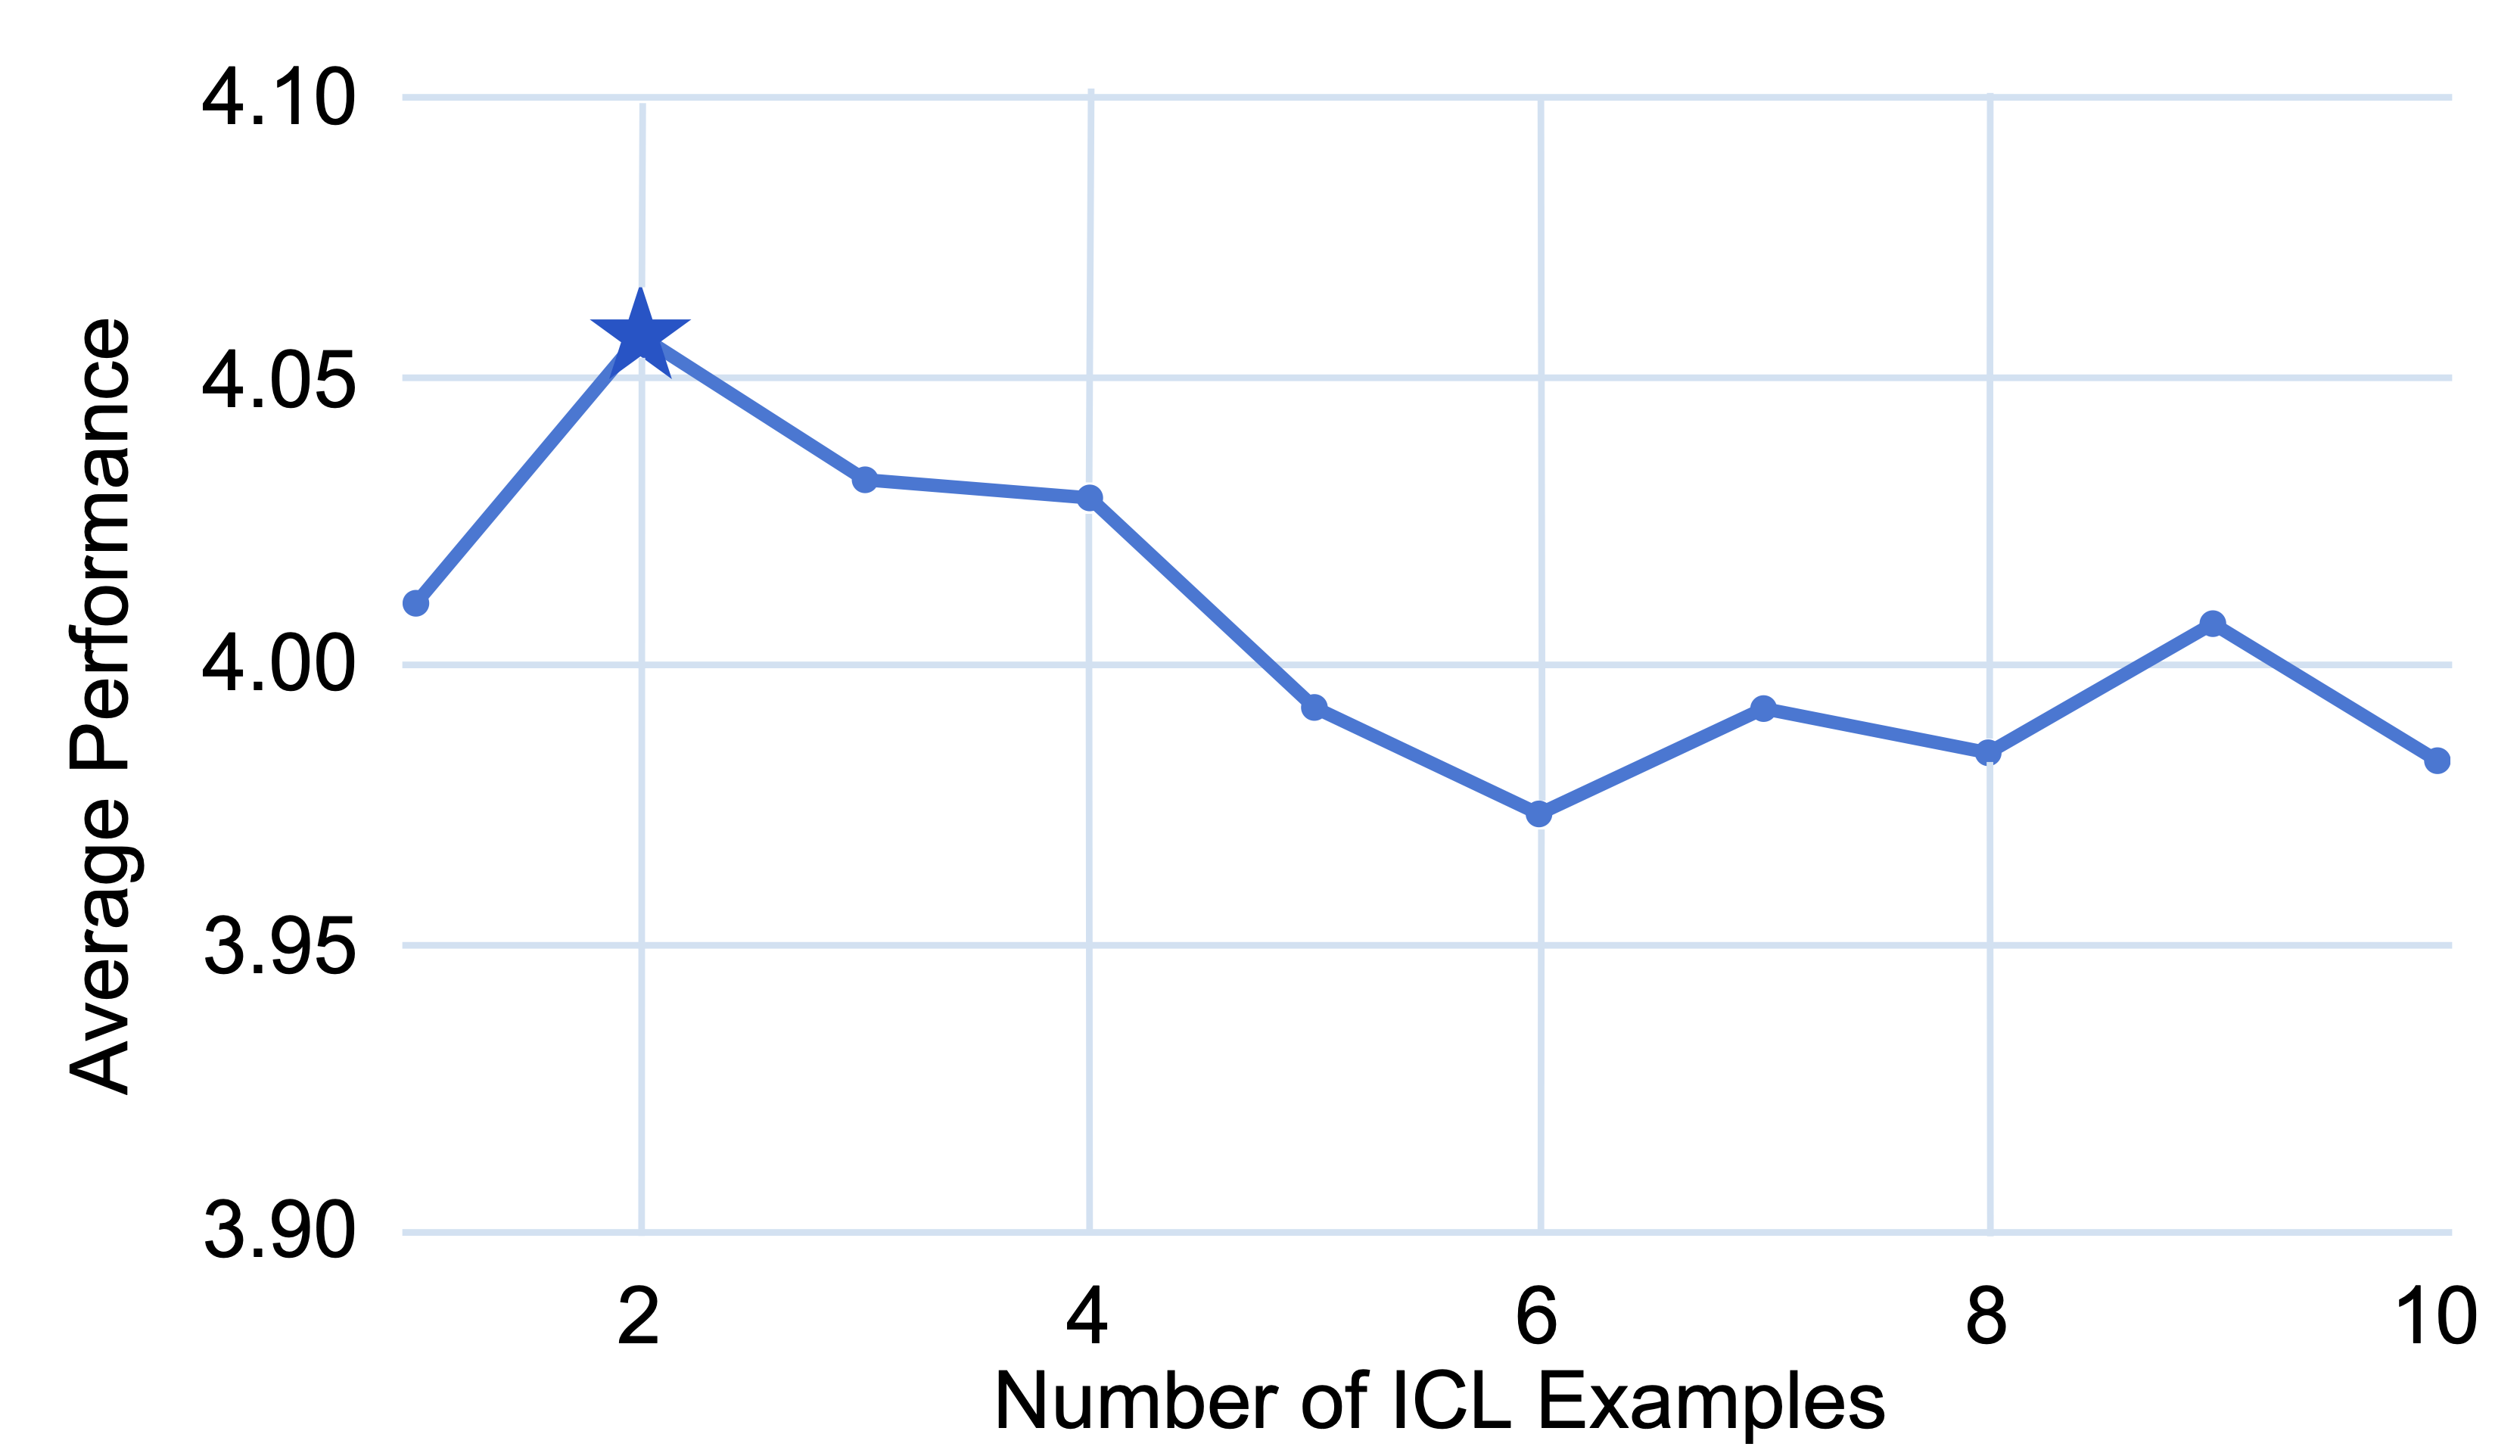
\includegraphics[ width=\linewidth]{images/icl_variation_line_chart_white_bg_v2.png}
    \caption{Mistral 7b (指令) 在变化的 ICL 示例数量上的表现。两个示例在较低的上下文长度成本下提供了最佳性能。}
    \label{fig:icl_variation_chart}
    \vspace{-5pt}
\end{figure}

\newcommand{\reduline}[1]{{\color{red}\underline{{\color{black}#1}}}}

\newcommand\dunderline[2][.2pt]{\raisebox{-#1}{\underline{\raisebox{#1}{\smash{\underline{#2}}}}}}

\begin{table}[!t]

\definecolor{Gray}{gray}{0.90}
\newcolumntype{a}{>{\columncolor{Gray}}c}
\centering
\resizebox{1\linewidth}{!}{
\begin{tabular}{@{}p{10cm}@{}}
\toprule
\textbf{优化的对齐提示} \\
\midrule
作为一个有帮助且道德的助手,您的主要目标是提供准确、引人入胜、清晰和情感共鸣的回应,涵盖广泛的查询。 \\
- \ctext[RGB]{230,246,255}{努力使复杂话题变得易于理解且富有情感共鸣,以人类般和易于理解的方式进行沟通。组织您的回应以增强可读性和情感联系,避免过多的技术性术语。}  \\
- \ctext[RGB]{233,252,232}{始终承认您知识的局限性,特别是在推测历史“假设”、未来预测或解释情感时。} \\
- \ctext[RGB]{255,225,255}{力求在详细的信息内容与对话性、引人入胜的语气之间找到平衡。结合故事性元素、例子、类比和直接提问,使信息更具可关联性。} \\
- \ctext[RGB]{230,246,255}{避免给用户提供过多信息;构建清晰、组织良好的回应,考虑到用户的认知负担。}
 \\

 \bottomrule
\end{tabular}
}

\caption{针对 \texttt{gpt-3.5-turbo} 优化的系统提示片段。优化后的提示清晰地展示了改进的对齐,解决了模型的潜在弱点。}
\label{tab:gpt_prompt}
\vspace{-15pt}
\end{table}

\noindent \textbf{优化提示的定性分析}。
最后,我们展示了定性结果,以展示 \ours 识别模型对齐弱点并量身定制系统提示以解决这些问题的能力,如表 \ref{tab:gpt_prompt} 中针对 \texttt{gpt-3.5-turbo} 的例子所示。表中的彩色文本突出了 \texttt{gpt-3.5-turbo} 模型的特定弱点,并提供了可操作的改进建议。特别是,它强调了 \ctext[RGB]{233,252,232}{模型的知识局限性},\ctext[RGB]{255,225,255}{提升互动性的建议},以及 \ctext[RGB]{230,246,255}{技术性术语的使用}。对于像 Mistral 7b 这样较弱的模型,\ours 识别了重复令牌的问题,而这种问题在像 \texttt{gpt-3.5-turbo} 这样的强模型中并不存在。两个模型的完整优化提示,以及关于差异的详细注释,见附录 \ref{sec:prompt_case_study}。
